\documentclass{article}
\usepackage[margin=1in]{geometry}
\usepackage[linesnumbered,ruled,vlined]{algorithm2e}
\usepackage{amsfonts}
\usepackage{amsmath}
\usepackage{amssymb}
\usepackage{amsthm}
\usepackage{enumitem}
\usepackage{fancyhdr}
\usepackage{hyperref}
\usepackage{minted}
\usepackage{multicol}
\usepackage{pdfpages}
\usepackage{standalone}
\usepackage[many]{tcolorbox}
\usepackage{tikz-cd}
\usepackage{transparent}
\usepackage{xcolor}
% \tcbuselibrary{minted}

\author{Nathan Solomon}

\newcommand{\fig}[1]{
    \begin{center}
        \includegraphics[width=\textwidth]{#1}
    \end{center}
}

% Math commands
\renewcommand{\d}{\mathrm{d}}
\DeclareMathOperator{\id}{id}
\DeclareMathOperator{\im}{im}
\DeclareMathOperator{\proj}{proj}
\DeclareMathOperator{\Span}{span}
\DeclareMathOperator{\Tr}{Tr}
\DeclareMathOperator{\tr}{tr}
\DeclareMathOperator{\ad}{ad}
\DeclareMathOperator{\ord}{ord}
%%%%%%%%%%%%%%% \DeclareMathOperator{\sgn}{sgn}
\DeclareMathOperator{\Aut}{Aut}
\DeclareMathOperator{\Inn}{Inn}
\DeclareMathOperator{\Out}{Out}
\DeclareMathOperator{\stab}{stab}

\newcommand{\N}{\ensuremath{\mathbb{N}}}
\newcommand{\Z}{\ensuremath{\mathbb{Z}}}
\newcommand{\Q}{\ensuremath{\mathbb{Q}}}
\newcommand{\R}{\ensuremath{\mathbb{R}}}
\newcommand{\C}{\ensuremath{\mathbb{C}}}
\renewcommand{\H}{\ensuremath{\mathbb{H}}}
\newcommand{\F}{\ensuremath{\mathbb{F}}}

\newcommand{\E}{\ensuremath{\mathbb{E}}}
\renewcommand{\P}{\ensuremath{\mathbb{P}}}

\newcommand{\es}{\ensuremath{\varnothing}}
\newcommand{\inv}{\ensuremath{^{-1}}}
\newcommand{\eps}{\ensuremath{\varepsilon}}
\newcommand{\del}{\ensuremath{\partial}}
\renewcommand{\a}{\ensuremath{\alpha}}

\newcommand{\abs}[1]{\ensuremath{\left\lvert #1 \right\rvert}}
\newcommand{\norm}[1]{\ensuremath{\left\lVert #1\right\rVert}}
\newcommand{\mean}[1]{\ensuremath{\left\langle #1 \right\rangle}}
\newcommand{\floor}[1]{\ensuremath{\left\lfloor #1 \right\rfloor}}
\newcommand{\ceil}[1]{\ensuremath{\left\lceil #1 \right\rceil}}
\newcommand{\bra}[1]{\ensuremath{\left\langle #1 \right\rvert}}
\newcommand{\ket}[1]{\ensuremath{\left\lvert #1 \right\rangle}}
\newcommand{\braket}[2]{\ensuremath{\left.\left\langle #1\right\vert #2 \right\rangle}}

\newcommand{\catname}[1]{{\normalfont\textbf{#1}}}

\newcommand{\up}{\ensuremath{\uparrow}}
\newcommand{\down}{\ensuremath{\downarrow}}

% Custom environments
\newtheorem{thm}{Theorem}[section]

\definecolor{probBackgroundColor}{RGB}{250,240,240}
\definecolor{probAccentColor}{RGB}{140,40,0}
\newenvironment{prob}{
    \stepcounter{thm}
    \begin{tcolorbox}[
        boxrule=1pt,
        sharp corners,
        colback=probBackgroundColor,
        colframe=probAccentColor,
        borderline west={4pt}{0pt}{probAccentColor},
        breakable
    ]
    \color{probAccentColor}\textbf{Problem \thethm.} \color{black}
} {
    \end{tcolorbox}
}

\definecolor{exampleBackgroundColor}{RGB}{212,232,246}
\newenvironment{example}{
    \stepcounter{thm}
    \begin{tcolorbox}[
      boxrule=1pt,
      sharp corners,
      colback=exampleBackgroundColor,
      breakable
    ]
    \textbf{Example \thethm.}
} {
    \end{tcolorbox}
}

\definecolor{propBackgroundColor}{RGB}{255,245,220}
\definecolor{propAccentColor}{RGB}{150,100,0}
\newenvironment{prop}{
    \stepcounter{thm}
    \begin{tcolorbox}[
        boxrule=1pt,
        sharp corners,
        colback=propBackgroundColor,
        colframe=propAccentColor,
        breakable
    ]
    \color{propAccentColor}\textbf{Proposition \thethm. }\color{black}
} {
    \end{tcolorbox}
}

\definecolor{thmBackgroundColor}{RGB}{235,225,245}
\definecolor{thmAccentColor}{RGB}{50,0,100}
\renewenvironment{thm}{
    \stepcounter{thm}
    \begin{tcolorbox}[
        boxrule=1pt,
        sharp corners,
        colback=thmBackgroundColor,
        colframe=thmAccentColor,
        breakable
    ]
    \color{thmAccentColor}\textbf{Theorem \thethm. }\color{black}
} {
    \end{tcolorbox}
}

\definecolor{corBackgroundColor}{RGB}{240,250,250}
\definecolor{corAccentColor}{RGB}{50,100,100}
\newenvironment{cor}{
    \stepcounter{thm}
    \begin{tcolorbox}[
        enhanced,
        boxrule=0pt,
        frame hidden,
        sharp corners,
        colback=corBackgroundColor,
        borderline west={4pt}{0pt}{corAccentColor},
        breakable
    ]
    \color{corAccentColor}\textbf{Corollary \thethm. }\color{black}
} {
    \end{tcolorbox}
}

\definecolor{lemBackgroundColor}{RGB}{255,245,235}
\definecolor{lemAccentColor}{RGB}{250,125,0}
\newenvironment{lem}{
    \stepcounter{thm}
    \begin{tcolorbox}[
        enhanced,
        boxrule=0pt,
        frame hidden,
        sharp corners,
        colback=lemBackgroundColor,
        borderline west={4pt}{0pt}{lemAccentColor},
        breakable
    ]
    \color{lemAccentColor}\textbf{Lemma \thethm. }\color{black}
} {
    \end{tcolorbox}
}

\definecolor{proofBackgroundColor}{RGB}{255,255,255}
\definecolor{proofAccentColor}{RGB}{80,80,80}
\renewenvironment{proof}{
    \begin{tcolorbox}[
        enhanced,
        boxrule=1pt,
        sharp corners,
        colback=proofBackgroundColor,
        colframe=proofAccentColor,
        borderline west={4pt}{0pt}{proofAccentColor},
        breakable
    ]
    \color{proofAccentColor}\emph{\textbf{Proof. }}\color{black}
} {
    \qed \end{tcolorbox}
}

\definecolor{noteBackgroundColor}{RGB}{240,250,240}
\definecolor{noteAccentColor}{RGB}{30,130,30}
\newenvironment{note}{
    \begin{tcolorbox}[
        enhanced,
        boxrule=0pt,
        frame hidden,
        sharp corners,
        colback=noteBackgroundColor,
        borderline west={4pt}{0pt}{noteAccentColor},
        breakable
    ]
    \color{noteAccentColor}\textbf{Note. }\color{black}
} {
    \end{tcolorbox}
}


\fancyhf{}
\setlength{\headheight}{24pt}

\date{\today}
\title{Math 115B Homework \#8}

\begin{document}
\maketitle

\begin{prob}
\end{prob}
\begin{enumerate}[label=(\alph*)]
    \item $H$ is a bilinear form, because $H(f,g)=H(g,f)$ and $H$ is linear in the first argument (therefore also the second). If $a \in \R$ and $f,g,h \in C([0,1])$, then
        \[ H(af+h,g)=\int_0^1 (af(x)+h(x))g(x) \d x = a \left( \int_0^1 f(x) g(x) \d x \right) +\left( \int_0^1 h(x)g(x) \d x \right) = aH(f,g)+H(h,g). \]
    \item $H$ is not a bilinear form, because if we let $v,w$ be vectors such that $J(v,w) \neq 0$, then $H(v,w)$ is also nonzero, which implies \begin{align*}
            H(v+v,w) &= (J(v,w)+J(v,w))^2 \\
                     &= H(v,w)+H(v,w)+H(v,w)+H(v,w) \\
                     &= (1+1)(H(v,w)+H(v,w)) \\
                     &\neq H(v,w)+H(v,w).
    \end{align*}
\item $H$ is not a bilinear form, because $H(1, 0)=1$, but linearity in the second argument would imply $H(x, 0)=0$ for any $x \in \R$.
\item This is a bilinear form, because it gives the determinant of the $2 \times 2$ matrix whose columns are the two parameters, and theorem 4.12 states that the determinant is the unique $n$-linear alternating function from $M_{n \times n}(F)$ to $F$ whish maps $I_n$ to 1. Therefore, the determinant of a $2 \times 2$ matrix can be thought of as a bilinear form on its rows, or equivalently, on its columns.
\item This is a bilinear form. We defined an inner product to be linear in the second argument (first, if you use silly math notation) and conjugate-linear in the first argument (second, if you never bothered to learn quantum mechanics). Since the underlying field of $V$ is $\R$, $H$ is linear in both arguments.
\item $H$ is not a bilinear form, because if $v, w \neq 0$, then
    \[ H(iv, w) = \mean{iv, w} = -i \mean{v, w} = -i H(v, w) \neq i H(v,w). \]
\end{enumerate}

\bigskip
\par
\begin{prob}
\end{prob}
\begin{enumerate}[label=(\alph*)]
    \item If $\alpha \in k$ and $H_1, H_2 \in \mathbb{B}(V)$, then $H_1$ and $H_2$ are both linear in the first argument. Linear combinations of linear functions are linear functions, so $H_1+H_2$ and $\alpha H_1$ are also linear in the first argument. By the exact same logic, they're linear in the second argument, so $H_1+H_2$ and $\alpha H_1$ are bilinear forms, which implies $\mathbb{B}(V)$ is a vector space (over $k$).
    \item Theorem 6.32 states that there is an isomorphism from $\mathbb{B}(V)$ and $M_{n \times n}(F)$, where $V$ is an $n$-dimensional vector space over $F$. Therefore the dimension of $\mathbb{B}(V)$ is $n^2$.
\end{enumerate}

\bigskip
\par
\begin{prob}
\end{prob}
Since we're given that $H$ is symmetric, $H(v,w)=H(w,v)$, so
\begin{align*}
    K(v+w)-K(v)-K(w)&=H(v+w,v+w)-H(v,v)-H(w,w) \\
                    &= \left[ H(v,v)+H(v,w)+H(w,v)+H(w,w) \right] - H(v,v)-H(w,w) \\
                    &= H(v,w) + H(w,v) \\
                    &= (1+1)H(v,w).
\end{align*}
Since $k$ does not have characteristic 2, we can divide both sides by 2 to get
\[ H(v,w) = \frac{1}{2} \left( K(v+w)-K(v)-K(w) \right). \]

\bigskip
\par
\begin{prob}
\end{prob}
\begin{enumerate}[label=(\alph*)]
    \item For any $u,v,w \in V$ and $\alpha \in \R$, we can see that $H$ is linear in the first argument because
        \[ H(\alpha v + u, w) = \mean{\alpha v + u, Tw} = \alpha^* \mean{v, Tw} + \mean{u, Tw} = \alpha H(v, w) + H(u, w), \]
        and it's linear in the second argument because
        \[ H(v, \alpha w + u) = \mean{v, T(\alpha w + u)} = \mean{v, \alpha Tw + Tu} = \alpha \mean{v, Tw} + \mean{v, Tu} = \alpha H(v,w) + H(v,u). \]
    \item $T^*$ is the unique operator such that $\mean{v, Tw}=\mean{T^*v, w}$ for all $v, w \in V$, so $T$ is Hermitian iff $\mean{v, Tw} = \mean{Tv, w}$ for all $v, w \in V$. Since $V$ is a real vector space, $\mean{Tv, w}=\mean{w, Tv}$, so that's equivalent to saying $\mean{v, Tw} = \mean{w, Tv}$, which is equivalent to saying $H(v,w)=H(w,v)$. Therefore $H$ is symmetric iff $T$ is Hermitian.
\end{enumerate}

\bigskip
\par
\begin{prob}
\end{prob}
Let $\mathcal{B} = (e_1, e_2, \dots, e_n)$ be an orthonormal basis for $V$, and let $A = \psi_\mathcal{B}(H)$ be the matrix representation of $H$ in that basis.
\par
Suppose $H(v,w)=\mean{v, Tw}$ for all $v,w \in V$. Then we can let $v=e_i$ and $w=e_j$ be basis vectors, so that $H(v,w)=A_{i,j}$, which implies $A_{i,j} = \mean{e_i, T e_j}$. But $\mean{e_i, T e_j}$ is just the $(i,j)$th entry of $[T]_\mathcal{B}$. Therefore $T$ is the linear operator such that $[T]_\mathcal{B} = A$, which means $T$ exists and is unique.


\bigskip
\par
\begin{prob}
\end{prob}
Suppose for the sake of contradiction that $p$ is not prime, so it is composite. Then there exist smaller positive integers $a, b$ such that $ab=p$. By the distributive rule,
\[ \left( \sum_{i=1}^a 1 \right) \left( \sum_{i=1}^b 1 \right) = \sum_{i=1}^p 1 = 0. \]
Since a field has no nonzero divisors of zero, either the sum of $a$ ones is zero, or the sum of $b$ ones is zero. But either of those cases would contradict the assumption that $p$ is the smallest positive integer for which
\[ \sum_{i=1}^p 1 = 0. \]
Therefore $p$ must be prime.


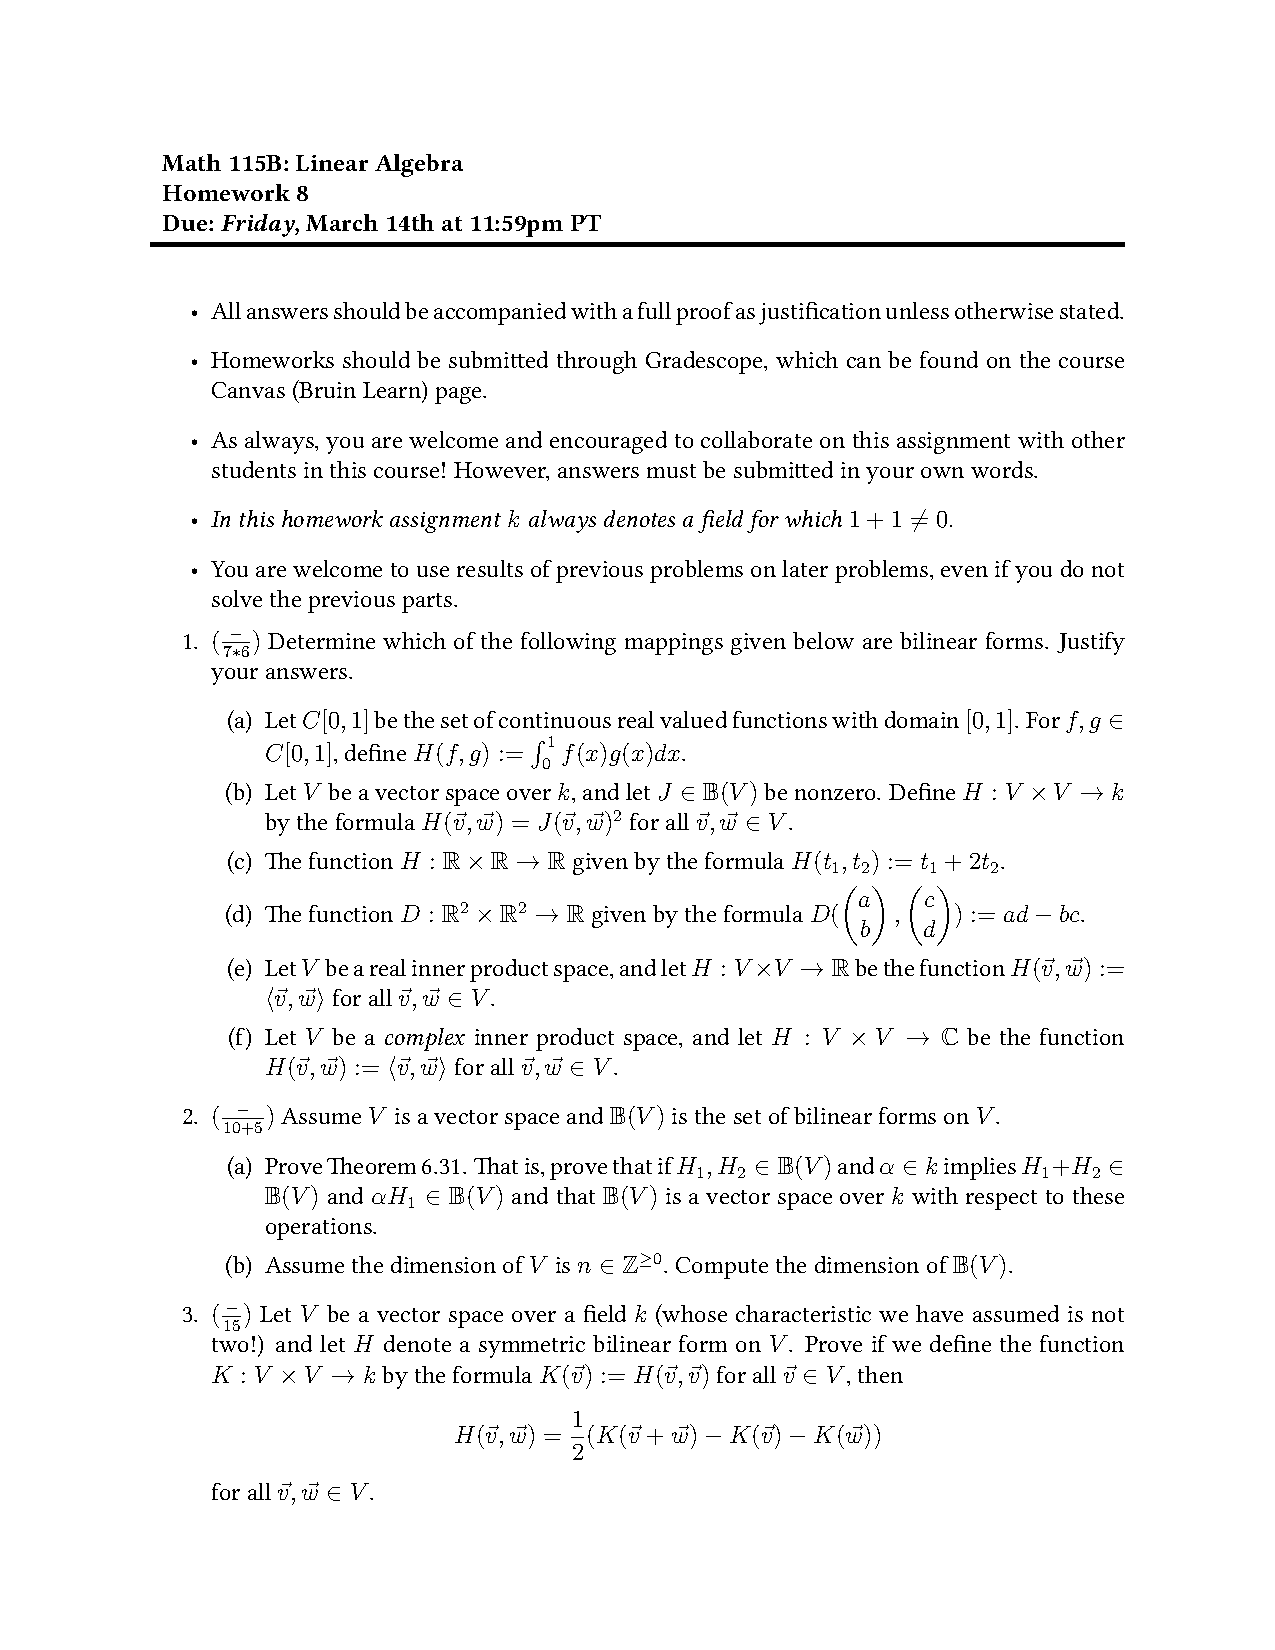
\includepdf[pages=-]{assignment.pdf}

\end{document}
